\documentclass{article}
% option ``report'' puts title on separate page

\usepackage{amsmath}
\usepackage[pdftex]{graphicx}

\begin{document}

\title{WS2: Finite Differencing and Interpolation}
\author{Jackie Villadsen}
\date{\today}
\maketitle


\section{Finite Difference Approximation and Convergence}
\subsection{Forward Differencing vs. Central Differencing}
I computed the first derivative of $f(x)=x^3-5x^2+x$ on the interval
[-2,6] using finite differencing and central differencing.
Figure \ref{fig:fwd} shows the error on the computed derivative using
forward differencing, where the error is the differencing between the
computed value of the derivative and the analytic value.  Two step sizes
were used to compute the derivative, dx=0.1 and dx=0.2.  Since central
differencing is first order, the errors for dx=0.1 are one half the errors
for dx=0.2.
\begin{figure}[h]
  \begin{center}
     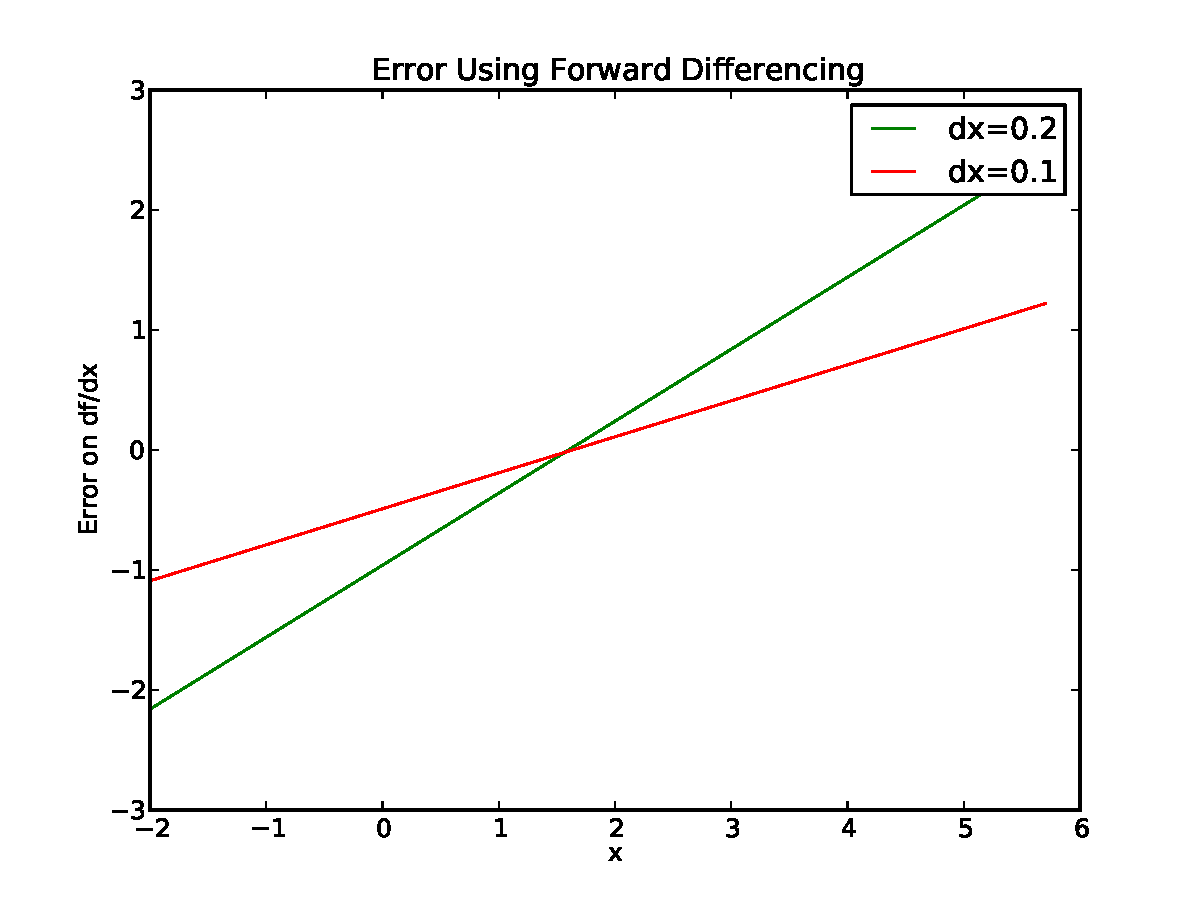
\includegraphics[width=\textwidth]{fwd}
  \end{center}
\caption{Error on the first derivative of $f(x)=x^3-5x^2+x$ computed
	 using forward differencing. The error on forward differencing
	 for step size $dx$ is $O(dx)$.}
  \label{fig:fwd}
\end{figure}

Figure \ref{fig:cen} shows the same quantities as Figure \ref{fig:fwd}, but
for central differencing.  Central differencing is second order, so the
errors for dx=0.1 are one quarter of the errors for dx=0.2.
\begin{figure}[h]
  \begin{center}
     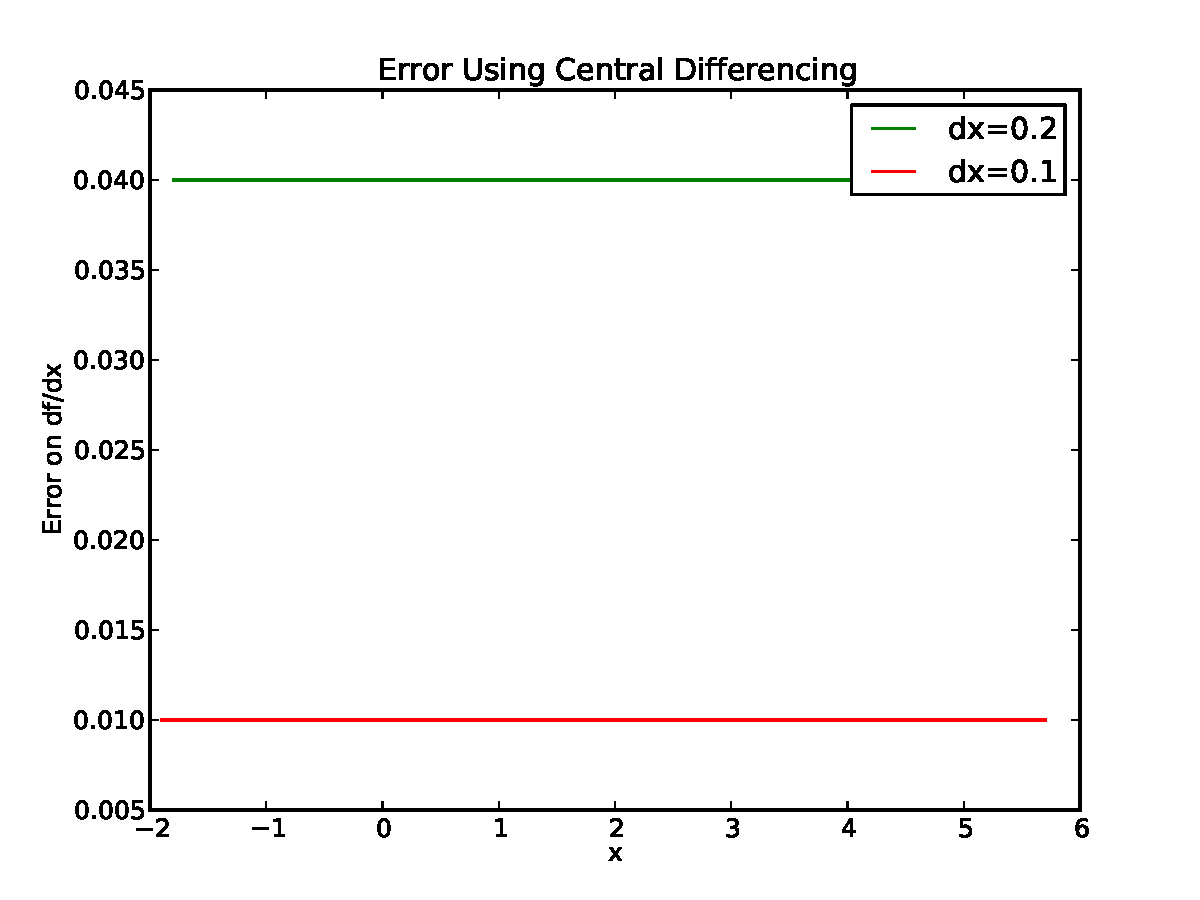
\includegraphics[width=\textwidth]{cen}
  \end{center}
  \caption{Error on the first derivative of $f(x)=x^3-5x^2+x$ computed
	   using central differencing. The error on central differencing
	   for step size $dx$ is $O(dx^2)$.}
  \label{fig:cen}
\end{figure}

\subsection{Finite Difference Estimate of the Second Derivative}
To get a central-differencing estimate for the second derivative of f, we start with
the Taylor expansions for $f(x_0+h)$ and $f(x_0-h)$:
\begin{equation}
	f(x_0+h) = f(x_0) + h f'(x_0) + \frac{h^2}{2} f''(x_0) + \frac{h^3}{6}f'''(x_0) + O(h^4)
\end{equation}
\begin{equation}
	f(x_0-h) = f(x_0) - h f'(x_0) - \frac{h^2}{2} f''(x_0) - \frac{h^3}{6}f'''(x_0) + O(h^4)
\end{equation}
By adding these two formulas and then solving for $f''(x_0)$, we get:
\begin{equation}
	f''(x_0) = \frac{f(x_0+h) - 2 f(x_0) + f(x_0-h)}{h^2} + O(h^2)
\end{equation}


\section{Interpolation: Cepheid Lightcurve}
Figure \ref{fig:ceph} shows the measured lightcurve of a Cepheid variable star with
a period of one day (measurements denoted by asterisks).  The same figure also shows
3 methods of interpolation: Lagrange interpolation (an n=8 polynomial fit using all 9
data points), piecewise linear interpolation, and piecewise quadratic interpolation.
The piecewise quadratic interpolation uses 3 data points to interpolate a magnitude $p(t)$
at time $t$.  I chose to use the two nearest data points at time less than or equal to $t$,
plus the nearest data point at time greater than $t$.  The n=8 polynomial has very large
errors far from the center of the data.  The piecewise linear and quadratic interpolation
both have sharp changes in derivative where the interpolated segments meet at the data points.

Figure \ref{fig:ceph2} shows 2 additional methods of interpolation: piecewise cubic Hermite
interpolation, and spline interpolation.  The Hermite interpolation improves upon the
previous methods since it accounts for the derivative at the data points.  However, the
spline provides the smoothest fit.

For all the methods except the n=8 polynomial, I took advantage of the periodicity of the
data by extending the data set by one period (repeating the same values) on either end of
the range of the interest from 0 to 1 days, in order to avoid dealing with edge effects.
If I do this for the polynomial, and increase the degree to be one less than the number of
data points (including those repeated), it looks much improved but still has some alarming wiggles.

\begin{figure}[h]
  \begin{center}
     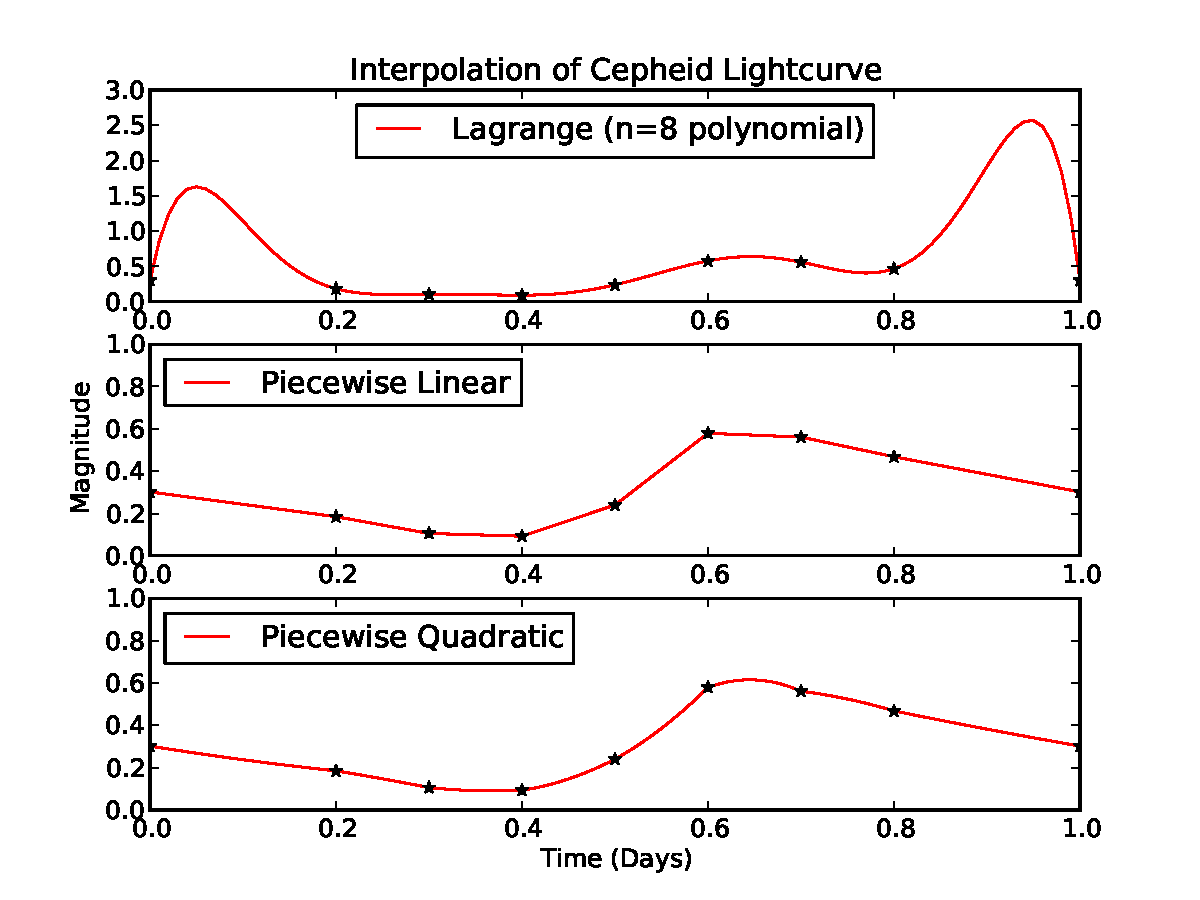
\includegraphics[width=\textwidth]{ceph}
  \end{center}
  \caption{Cepheid lightcurve with a period of one day.  3 methods of interpolation
	   shown: Lagrange (n=8 polynomial) interpolation, piecewise linear interpolation,
		  and piecewise quadratic interpolation.}
  \label{fig:ceph}
\end{figure}

\begin{figure}[h]
  \begin{center}
     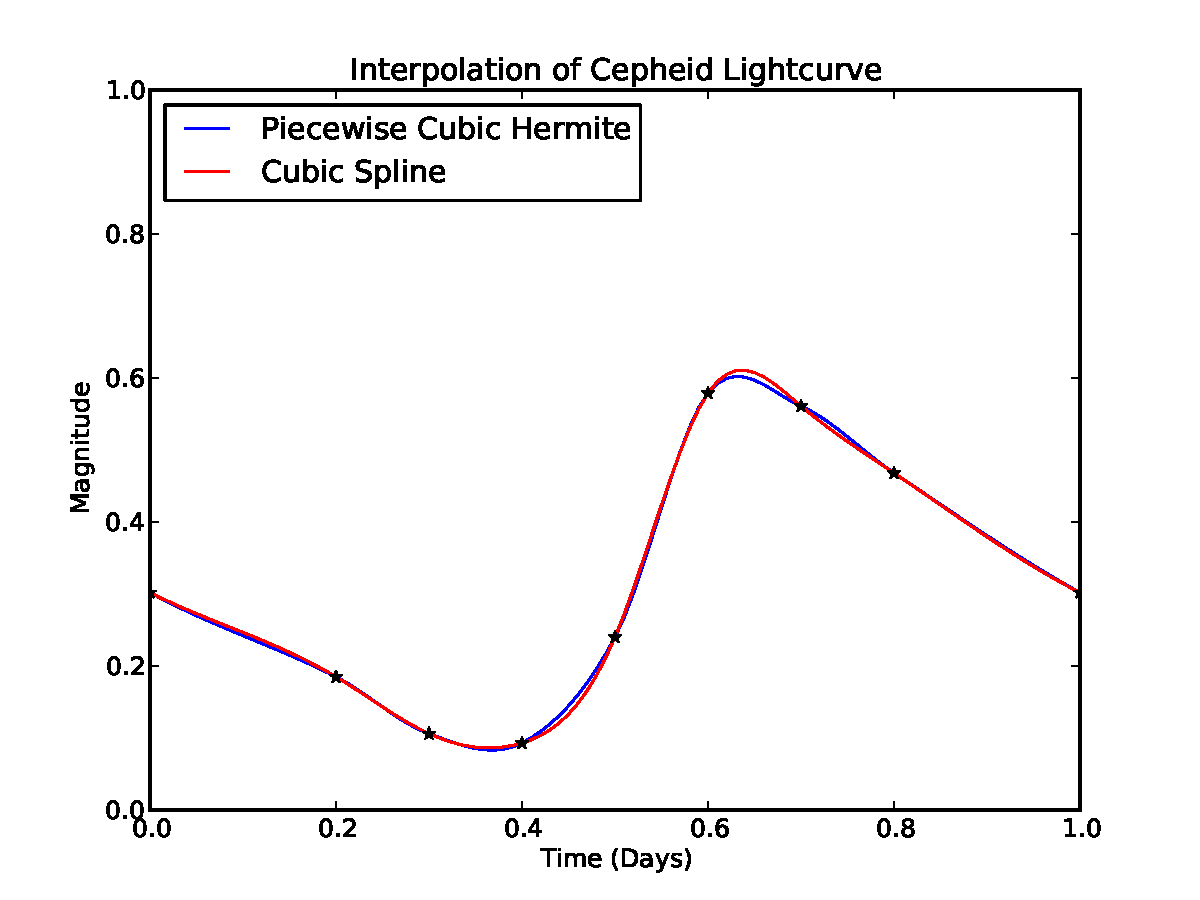
\includegraphics[width=\textwidth]{ceph2}
  \end{center}
  \caption{Cepheid lightcurve with a period of one day.  2 methods of interpolation
	   shown: Piecewise cubic Hermite interpolation, and cubic spline interpolation.}
  \label{fig:ceph2}
\end{figure}

\end{document}
